\lstset{style=langstyle}
\section{Mutation Analysis}

Attempting to improve a fuzzing effort is one way to find problems
with the effort; if you succeed, you found a weakness.  However, none
of the attempts described above exposed a serious problem.  Adding more fuzzers would
be \emph{good}, but was not obviously \emph{essential}.  True ensemble
fuzzing was not feasible, and swarm testing was, for practical
purposes, already performed by alternative means.  An alternative is
to directly look for holes in testing.  The Bitcoin Core fuzzing team
clearly was measuring and inspecting code coverage (see \url{https://marcofalke.github.io/btc_cov/}), so little value
would be added by inspecting traditional coverage alone.  Mutation
testing/analysis~\cite{MutationSurvey,budd1979mutation,demillo1978hints}, however, subsumes code coverage and adds extremely
valuable information on \emph{oracle power} in addition to mere
coverage~\cite{Discontents}.  This is perhaps especially valuable in fuzzing, where ``you
only see crashes'' is a persistent concern.  In previous work, we had
used mutation testing to improve the random testing of the Linux
kernel's RCU module, and in the process discovered some subtle kernel bugs~\cite{mutKernel,groce2018verified}.

\begin{sloppypar}
We used the universal mutator
\noindent(\url{https://github.com/agroce/universalmutator})~\cite{regexpMut}, a
mutation tool already used widely in the blockchain and smart contract world, to
mutate the Bitcoin Core transaction
verification code, and, subsequently, that of other popular cryptocurrencies. We focused on transaction verification/validation code, as it is generally well-covered by
tests, and obviously an extremely critical functionality for any blockchain.
\end{sloppypar}

\subsection{Mutation Testing Bitcoin}

\begin{sloppypar}

To perform mutation analysis on Bitcoin, we generated mutations for code in the
{\tt tx\_verify.cpp} file.  Fuzzing covers 96 of 98 lines of code, 8
of 8 functions, and 74 of 102 branches for this file, guaranteeing
that mutation testing will not primarily reflect missing coverage.
Comparing coverage to that for functional testing, the fuzz testing
has very slightly lower branch coverage, but the numbers are almost
identical (72.5\% vs. 73\%), and the fuzz testing covers \emph{different} branches than
the functional testing.  The missing lines are different for
functional and fuzz testing, as well, in fact.  And, as noted above,
there can be no doubt that transaction verification is a critical
Bitcoin function: in fact, arguably, checking transactions for
correctness is \emph{the raison d'être} of any blockchain, and getting
transactions that should be invalid past such checks would be an
obvious potential attacker goal.
We evaluated the ability of fuzzing and functional testing
to detect mutants of {\tt tx\_verify.cpp}. Figure~\ref{kills} summarizes our mutation
analysis of the file.

\begin{figure}
\vspace{2mm}
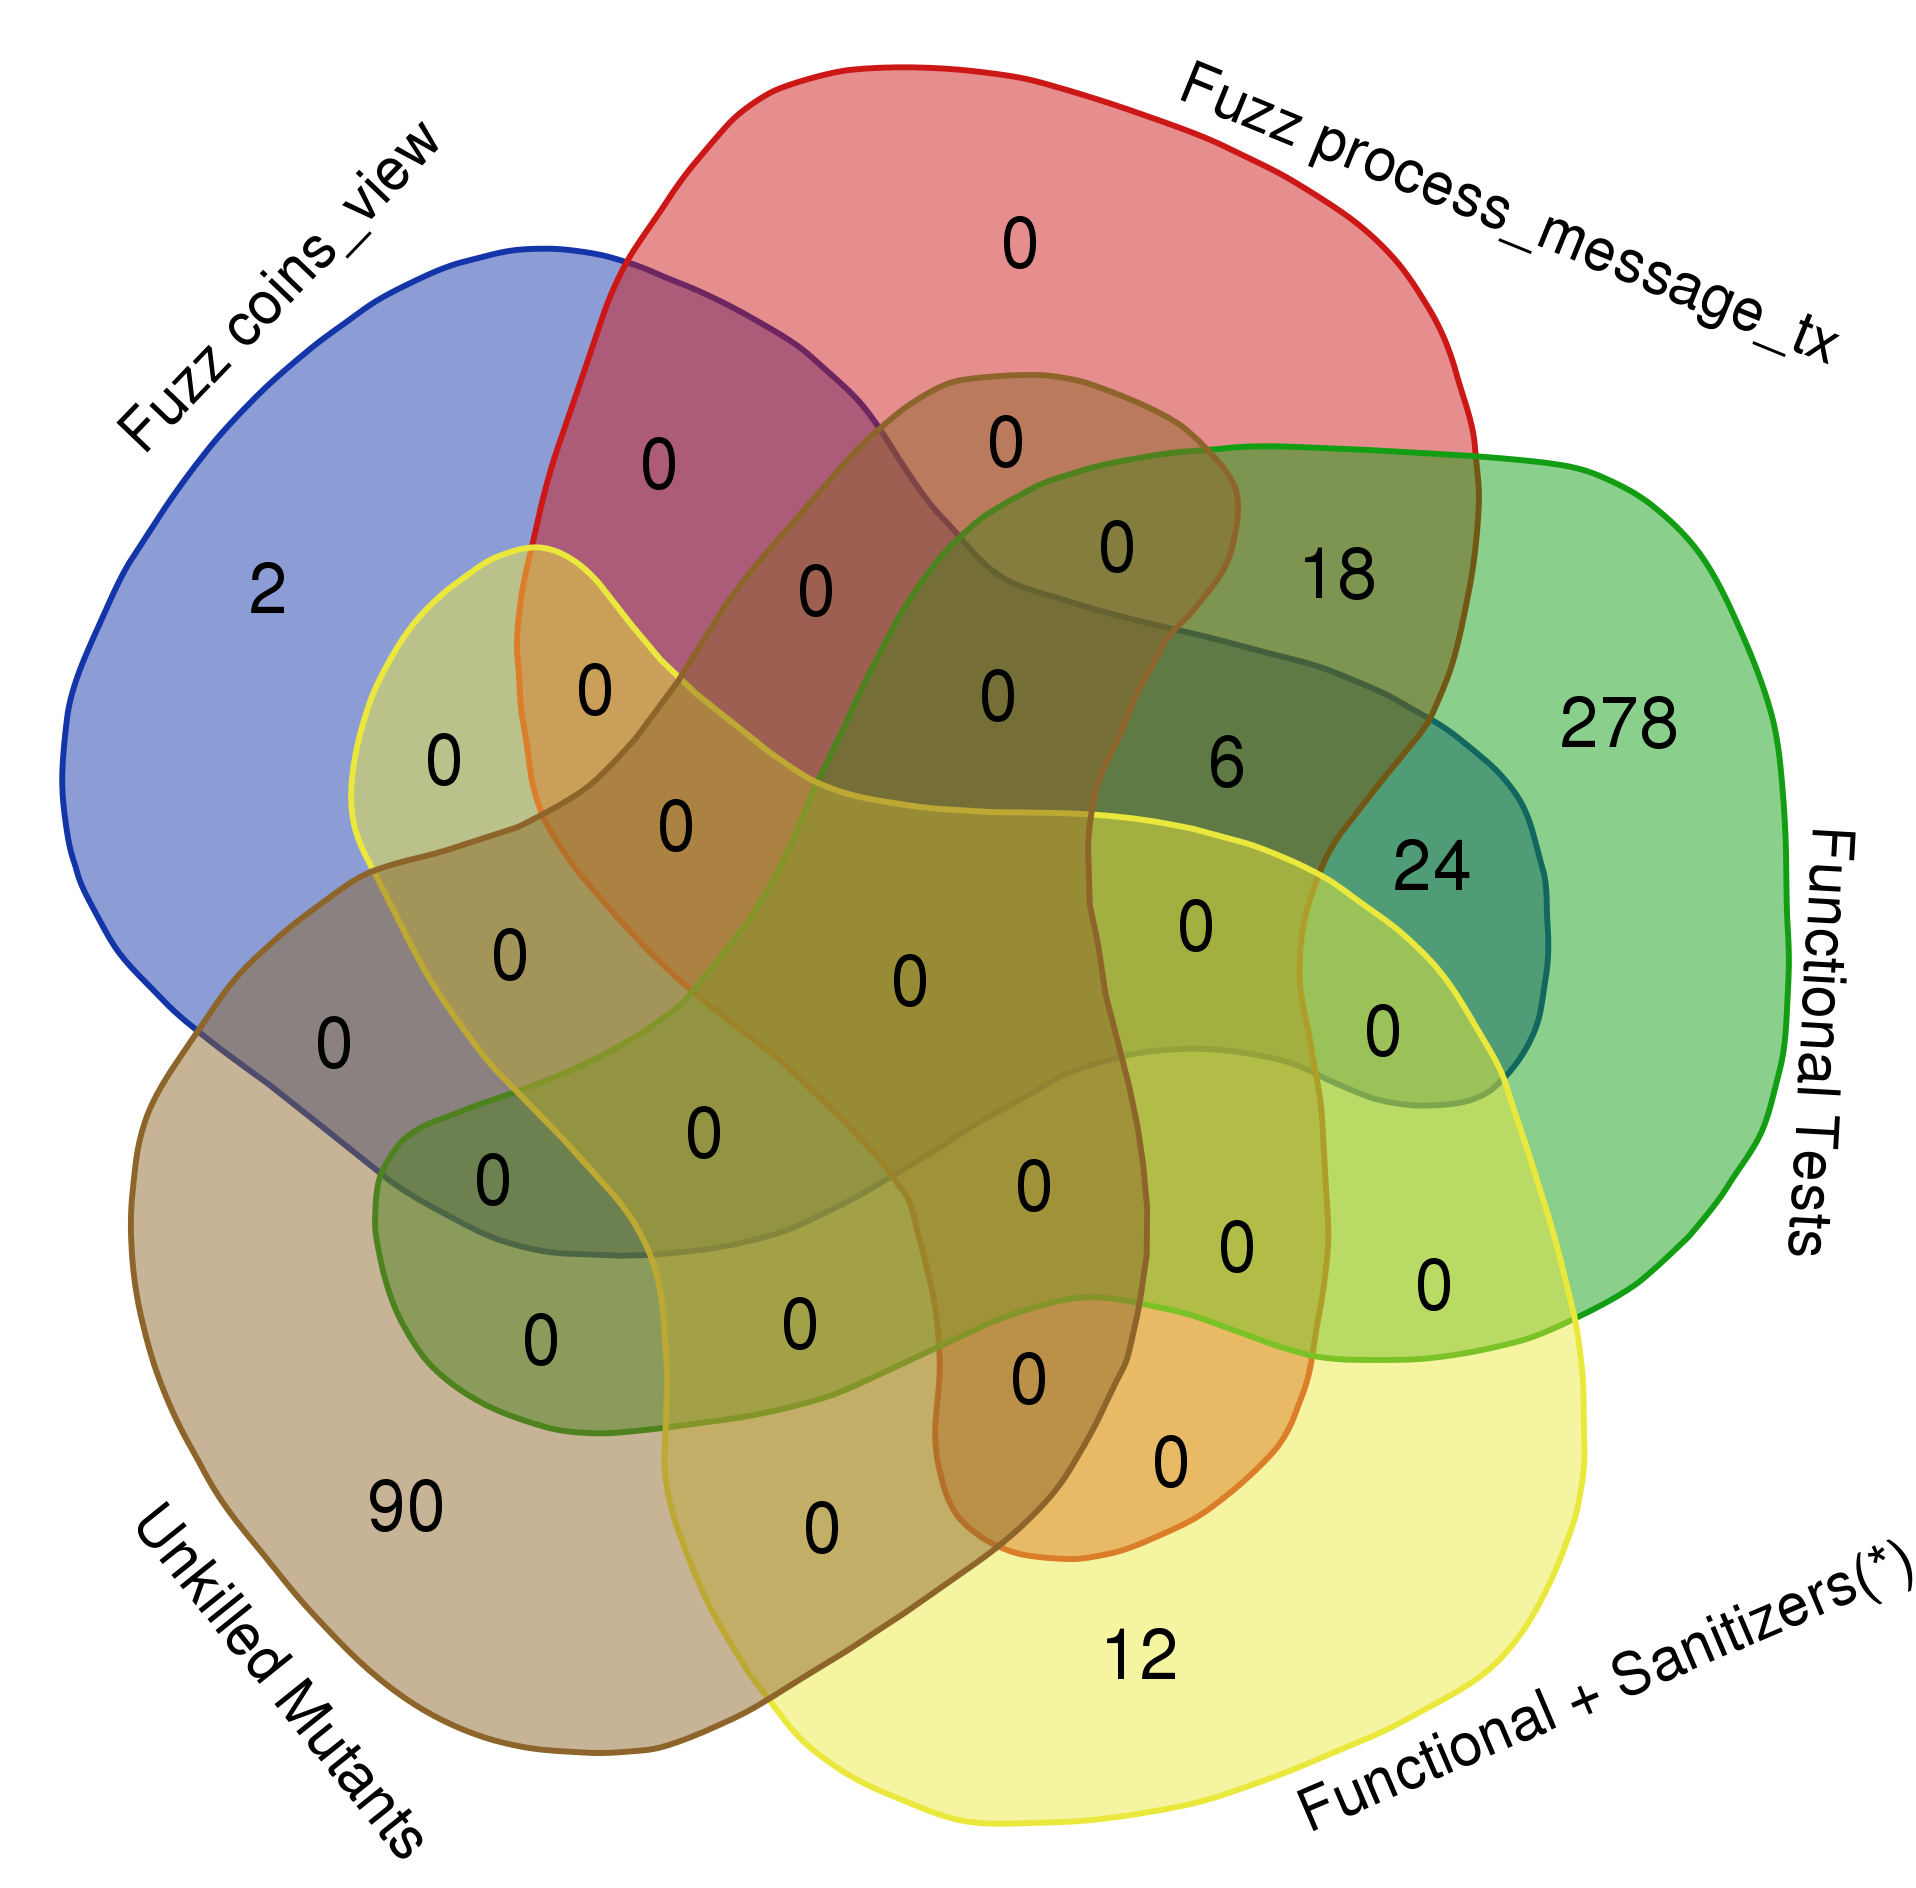
\includegraphics[width=0.9\columnwidth]{kill_pre_valgrind.png}
\caption{A comparison of mutation kills for {\tt tx\_verify.cpp} when
  subjected to different testing and fuzzing parameters.  At least 29
  of the 90 surviving mutants are equivalent, and thus not indicative
  of testing weaknesses.  * indicates
  only mutants not killed by other methods were analyzed;}
\label{kills}
\end{figure}

\begin{figure*}
\raggedright
{\scriptsize
{\bf Original mutated code (and immediate context):}

\begin{code}
    if (coin.IsCoinBase() \&\& nSpendHeight - coin.nHeight < COINBASE\_MATURITY) \{
            return state.Invalid(TxValidationResult::TX\_PREMATURE\_SPEND, "bad-txns-premature-spend-of-coinbase",
                strprintf("tried to spend coinbase at depth \%d", nSpendHeight - coin.nHeight));
\end{code}

{\bf Mutant \#379} changes the {\tt strprintf} to:

\begin{code}
strprintf("tried to spend coinbase at depth \%d", nSpendHeight / coin.nHeight));
\end{code}

{\bf Mutant \#380} changes the {\tt strprintf} to:

\begin{code}
strprintf("tried to spend coinbase at depth \%d", nSpendHeight \% coin.nHeight));
\end{code}
}
\caption{Mutants detected \emph{only} by fuzzing.}
\label{mkills}
\end{figure*}

The universal mutator generated 430 compiling mutants of the file in
less than three hours\footnote{Building all test and fuzz targets for each
candidate mutant takes some time, and parallelizing the task would
require multiple sandboxed copies of the code. Constructing a more
focused build command than {\tt make -j5}, that avoids building most tests, might speed this up substantially.}.
Two fuzz targets seemed to be relevant to fuzzing {\tt
  tx\_verify.cpp} code: {\tt process\_message\_tx} and {\tt coins\_view}.
In theory {\tt process\_message} and {\tt process\_messages} were
also potential interest, but the relevant corpus entries were
duplicated in {\tt process\_message\_tx} (we verified the two more
general targets provided \emph{no}
additional mutant kills). We ran fuzzing for five minutes using
libFuzzer exploration based on the full (and quite large: 4,517 tests for
{\tt process\_message\_tx}, and 6,889 for {\tt coins\_view}) QA asset corpus for each
harness, with all sanitizers enabled. The {\tt process\_message\_tx} target was
able to detect 24 mutants, and the {\tt coins\_view} harness was able to detect
32 mutants, for a total of 50 mutants (since some mutants were
detected by both). In other words, fuzzing could detect just under 12\%
of all the generated mutants. This is not necessarily a bad result: fuzzing inherently has
trouble detecting subtle, non-crash-inducing, bugs in code, because writing a
strong specification of correct behavior that covers all the bizarre and
pointless inputs produced in fuzzing is often impractical, or would require a
specification nearly as complex as the code itself. This is one reason
\emph{differential} fuzzing is promising: a reference implementation is such a
specification. Bitcoin Core's cryptographic elements are, in fact,
differentially fuzzed
\url{https://github.com/bitcoin/bitcoin/pull/22704#issuecomment-898989809}.
\end{sloppypar}


A major purpose of fuzzing is, then, to address limits in more
traditional functional testing, where known inputs are paired with
expected behavior.  While functional or unit testing is very powerful,
the kinds of bugs found in vulnerabilities often involve the kind of
inputs that don't appear in ``normal'' unit/functional tests, as shown
by the success of fuzzing and security audits~\cite{FC20}.  The real
question, then, is how many mutants that survive Bitcoin Core's
extensive functional tests survive fuzzing.

The answer is: not too many.  The functional tests without sanitizers
enabled catch an additional 278 mutants.  Turning on sanitizers (which
is very expensive --- we \emph{only} ran it for mutants surviving all other
tests, as indicated by the zero overlap and the asterisk in Figure~\ref{kills}) catches an additional 12 mutants.  Only 90 of the
430 compiling mutants survive all tests, for an overall mutation score
of 79.07\%.

Fuzzing adds two unique mutant kills beyond those produced by
the functional testing.  Figure~\ref{mkills} shows the (very similar
code) for these two mutants.  Only fuzzing generates inputs that cause
{\tt coin.nHeight} to be zero.  Fuzzing doesn't increase code coverage
here, but does increase interesting \emph{data value} coverage.  Use
of the libFuzzer {\tt -use\_value\_profile=1} flag is likely
instrumental in achieving such good value coverage.  Adding that flag was
one of the first suggestions in the 80 hour effort, but it turned out
this was already standard practice in the Bitcoin Core fuzz
configuration.  Note that the opportunity for either approach to
generate a zero value here is limited: functional tests only cover the
mutated line 14 times, and fuzzing 556 times.  In contrast, both cover
numerous other lines of code more than a million times.  For
functional tests, the line is the 2nd least-covered line executed in {\tt
  tx\_verify.cpp}, and it is the 4th least-covered line executed for fuzzing.

Manual inspection of the 90 surviving mutants showed that at
least 29 of these were clearly semantically equivalent to the
un-mutated code.  For instance, many mutants removed or weakened an
assertion; clearly this cannot ever be detected, since it can only
transform failing tests into passing tests.  The full, detailed list
of surviving, not-obviously-equivalent mutants, prioritized by an FPF ranking~\cite{10.1145/2491956.2462173,Gonzalez85}, is
available here:
\url{https://github.com/agroce/bitcorpus/blob/master/mutation/prioritized_full_inspect.txt}.
Discussion with the Bitcoin Core team is ongoing as we write
(\url{https://github.com/bitcoin/bitcoin/issues/22690}), but thus far
none of these mutants seem to expose serious testing
problems.  After manual pruning, the mutation score is 85.8\%, and
some of the remaining 61 mutants are likely also equivalent.  The
limitations of the fuzzing oracle are clear: fuzzing covers 98\% of
statements and 72.5\% of branches as we write, but can kill fewer than
12\% of mutants.  The much greater killing power of the functional
tests obviously does not lie in the marginal 0.5
percentage points of  branch coverage it obtains; it lies
in the ability to reject incorrect executions that do not crash or set
off a sanitizer alarm.

This raises the question:  why fuzz?  The coverage for high quality
(if imperfect) functional tests such as those for Bitcoin Core will
often be considerably
higher, and the oracle will almost always be \emph{much} more powerful.  The answer lies in the
fact that, even in the presence of such high quality tests, fuzzing
uncovers subtle bugs that functional tests designed by humans will
almost never detect,
e.g. \url{https://github.com/bitcoin/bitcoin/issues/22450}\footnote{Comments
  on this bug, such as ``Another win for fuzzing, oh wow.'' and
  ``Fuzzer rulez!'' show that the Bitcoin Core team has little doubt
  about the power of fuzzing.}.  In part this is due to the fact that
when functional tests and fuzzing have similar coverage, they often
cover \emph{different} hard-to-reach code, as in the case of {\tt
  tx\_verify.cpp}.  Fuzzing is \emph{not} a replacement
for functional/unit tests; and functional/unit tests are not a
replacement for fuzzing.  In our mutation analysis, consider the two
mutants detected by {\tt coins\_view} fuzzing alone.  In the
traditional, score-based, view of mutation analysis, the {\tt
  coins\_view} fuzz harness would be seen as performing badly.  But it
detects two (hypothetical) bugs not detectable by other means; in the
real world, if one such bug is exploitable, detecting it may ``pay
for'' all the fuzzing effort, and there will seldom be just one such
bug (see
\url{https://github.com/bitcoin/bitcoin/issues?q=is\%3Aissue+fuzz+is\%3Aclosed+label\%3ABug}
for an approximate list of fuzzer-detected, fixed bugs in Bitcoin
Core).  If the ``good guys'' don't fuzz well, you can be sure the bad
guys will, for software protecting billions of dollars of assets.

\subsection{Other Cryptocurrency Projects}


% for solana, these are app.codecov.io/gh/solana-labs/solana @a6a4cfd numbers. grcov
% doesn't include tests, but reports coverage % as a total over lines including
% tests, so it's also not accurate. we'll just over approximate rather than
% underapproximate and acknowledge that in the text
\begin{table*}[ht!]
\vspace{2mm}
\centering
\begin{tabular}{llrccc}
\toprule
\bf \mr{2}{Project}             & \bf \mr{2}{File path}                         & \bf \mr{2}{LOC}  & \mc{1}{c}{\bf Mutation} & \mc{1}{c}{\bf File}     & \mc{1}{c}{\bf Project}   \\
\bf                             & \bf                                           & \bf              & \mc{1}{c}{\bf score}    & \mc{1}{c}{\bf coverage} & \mc{1}{c}{\bf coverage}  \\
\midrule
bitcoin                         & src/consensus/tx\_verify.cpp                  & 210              & 78.6\%                  & 98.7\%                  & 84.2\%                   \\
\cmidrule{2-6}
\mr{3}{go-ethereum}             & core/block\_validator.go                      & 129              & 70.1\%                  & 81.0\%                  &  \mr{3}{58.8\%}          \\
                                & signer/fourbyte/validation.go                 & 127              & 49.5\%                  & 60.0\%                  &                          \\
                                & signer/core/signed\_data.go                   & 1,044            & 25.3\%                  & 69.3\%                  &                          \\
\cmidrule{2-6}
%\mr{3}{solana}                  & perf/src/sigverify.rs                         & 1,246            & ????\%                  & 74.48\%                 & \mr{3}{82.2\%}           \\
%                               & core/src/sigverify\_stage.rs                  & 296              & ????\%                  & 88.46\%                 & \mr{3}{82.2\%}           \\  this seems to just call perf/src/sigverify
%                                & core/src/validator.rs                         & 2,016            & -                       & 73.29\%                 &                          \\
%                                & core/src/tvu.rs                               &  494             & -                       & 63.12\%                 &                          \\
%\cmidrule{2-6}
dogecoin                        & src/bitcoin-tx.cpp                            & 847              & 58.7\%                  & -$^\dagger$               & 70.1\%                   \\
\cmidrule{2-6}
avalanchego                     & vms/platformvm/add\_subnet\_validator\_tx.go  & 308              & 57.3\%                  & 81.0\%                  & 63.6\%                   \\
\cmidrule{2-6}
  stellar                       & src/historywork/VerifyTxResultsWork.cpp       & 192              & 85.1\%                  & 85.3\%                  & 74.9\%                   \\
\cmidrule{2-6}
cosmos-sdk                      & x/auth/ante/sigverify.go                      & 510              & 67.3\%                  & 67.0\%                  & 60.9\%                   \\
\bottomrule
\end{tabular}
\caption{Code Coverage and Mutation Scores Across Popular Cryptocurrencies. \underline{Mutation score} represents the proportion of mutants that were killed divided by the total number of mutants (higher is better).
\underline{File coverage} and \underline{Project coverage} report statement level coverage for the file and entire project, respectively. \underline{LOC} represents the lines of code of the chosen file. $^\dagger$We were unable to obtain coverage for this file.
}
\label{tab:comparison}
\end{table*}


\begin{table*}[ht!]
\vspace{2mm}
\centering
\begin{tabular}{lll}
\toprule
\bf Mutation Operator                          & \bf Project and File                  & \bf Mutation Example   \\
\midrule
Comment out source code line                   & bitcoin - tx\_verify.cpp              &
\begin{lstlisting}[language=C2diff]
if (!MoneyRange(coin.out.nValue) || !MoneyRange(nValueIn)) {
-  return state.Invalid(TxValidationResult::TX_CONSENSUS,
-     "bad-txns-inputvalues-outofrange");
+  /* return state.Invalid(TxValidationResult::TX_CONSENSUS,
+     "bad-txns-inputvalues-outofrange"); */
}
\end{lstlisting}                               \\
Replace \texttt{<} with \texttt{==}                              & go-ethereum - block\_validator.go     &
\begin{lstlisting}[language=Godiff]
- if desiredLimit < params.MinGasLimit {
+ if desiredLimit == params.MinGasLimit {
  desiredLimit = params.MinGasLimit
}
\end{lstlisting}                               \\
Add continue to statement                      & dogecoin - bitcoin-tx.cpp              &
\begin{lstlisting}[language=C2diff]
while ((!feof(f)) && (!ferror(f))) {
  char buf[4096];
+ continue;
  ...
}
\end{lstlisting}                               \\
Add break to statement                         & bitcoin - tx\_verify.cpp               &
\begin{lstlisting}[language=C2diff]
for (const auto& txin : tx.vin) {
+ break;
  nSigOps += txin.scriptSig.GetSigOpCount(false);
}
\end{lstlisting}                              \\
Flip arguments of function                    & go-ethereum - validation.go             &
\begin{lstlisting}[language=Godiff]
if tx.Data != nil && tx.Input != nil
-       && !bytes.Equal(*tx.Data, *tx.Input) {
+       && !bytes.Equal(*tx.Input, *tx.Data) {
  return nil, errors.New(`...`)
}
\end{lstlisting}                               \\
\bottomrule
\end{tabular}
\caption{Sample of Mutation Rules and Examples for Various Cryptocurrencies that were not killed.}
\label{tab:rules}
\end{table*}

\begin{figure}
\vspace{2mm}
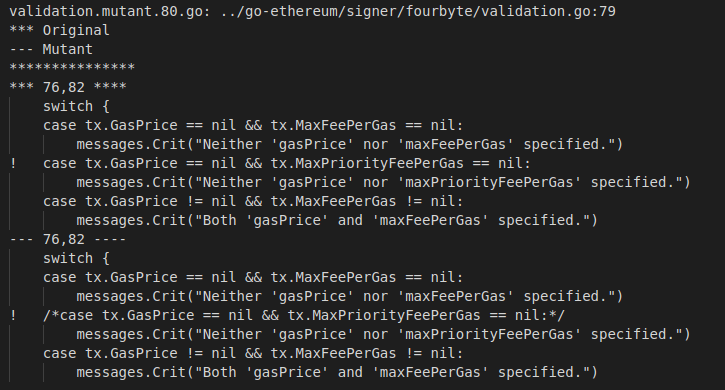
\includegraphics[width=0.9\columnwidth]{mutation-example.png}
\caption{A mutation for Ethereum transaction validation.}
\label{fig:mutation}
\end{figure}

\begin{figure}
\vspace{2mm}
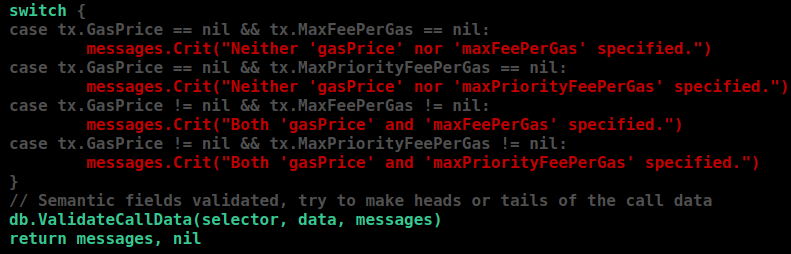
\includegraphics[width=0.9\columnwidth]{coverage-example.png}
\caption{Missed coverage for mutations in Figure~\ref{fig:mutation}.}
\label{fig:coverage}
\end{figure}

To put our work on Bitcoin in context, we performed mutation analysis
of transaction-verification-related code for other popular cryptocurrencies.
We generated mutants using the universal mutator for code in Ethereum,
Dogecoin, Avalanche, Stellar, and Cosmos implementations, a selection from the top 30
cryptocurrencies\footnote{We chose these by market capitalization according to
\url{https://coinmarketcap.com}.} Our selection was also influenced by the
availability of code coverage, and indicative of the opportunities for
mutation testing of Bitcoin and popular altcoins, rather than a
comprehensive survey. Because it requires significant effort to set up or
otherwise understand the extent of fuzz testing in this heterogeneous selection
of projects, our mutation analysis here only considers mutation testing
against the project test suite, not fuzzing.  As discussed above,
without heroic effort, fuzzing is likely to add only modest additional
mutant kills.

We identified candidate files that might be roughly comparable to
Bitcoin's {\tt tx\_verify.cpp} by searching for keywords like \texttt{transaction},
\texttt{verify}, \texttt{sign}, and \texttt{validate}. We manually inspected
functions and test coverage for these functions (where applicable) to identify
which files would be interesting targets for mutation. Ultimately we
settled on one to three files per project that are representative of some
interesting and tested functionality (a choice that we readily acknowledge is by
no means comprehensive or suggestive of a project's quality and testing as a
whole).

\subsubsection*{Setup}
We ran the universal mutator on the candidate files above, using both universal and
language specific rules. There were 92 universal rules (transformations that can apply to
any language) and between 0 and 20 language specific rules, depending on the project source language.\footnote{See \url{https://github.com/agroce/universalmutator/tree/master/universalmutator/static}}
Across all projects, our rules generated between 492 and 8,567 mutants per file.
% RVT says: think just the range is good enough, keeping the actual files in comments because it's good to know for ourselves.
% 492 (go-ethereum's {\tt block\_validator.go}) to
% 8567 (go-ethereum's {\tt signed\_data.go}) mutants.
We ran mutants against each project's default test suite (determined by consulting READMEs and build/CI documentation) using universal mutator to obtain a final mutation score. The runtime
of this step naturally varies depending on test suite execution speed and candidates per file, ranging from
42 minutes (go-ethereum's {\tt validation.go}) to 32 hours (dogecoin's
{\tt bitcoin-tx.cpp}).

\subsubsection*{Results.}
Table~\ref{tab:comparison} summarizes our results, and lists the
\textbf{Mutation score}, \textbf{File coverage}, and \textbf{Project coverage}. \textbf{Mutation score} represents the proportion of
generated mutants that were killed by the project's test suite divided by the total number
of mutants (higher is better). File and project metrics report statement level coverage
for each chosen file and the entire project. In principle, we expect that higher file coverage
(i.e., more tested code) should correlate with a higher mutation
score.

For illustration, Table~\ref{tab:rules} shows some of the mutation rules
with examples of surviving mutants. One commonly used operator,
statement deletion, comments out a
line of source code.
Other operators included adding {\tt break} and {\tt continue} to statements,
along with changing binary operators such as \texttt{<} to \texttt{==}.
Investigating files with lower coverage (e.g., those in Ethereum), we noticed
that many of the generated mutants removed lines related to error checking
(e.g., in switch statements) that were apparently not covered by tests (cf.
Figures \ref{fig:mutation} and \ref{fig:coverage}).

The Bitcoin Core mutation score (without pruning or fuzzer-killed
mutants) ranks high: 2nd out of 6 projects. Bitcoin Core
also has the highest File and Project coverage of any project.  Our experience
working with Bitcoin Core developers suggests that they are pro-active about code
quality and testing, which is likely to lead (directly or
indirectly) to test suite quality.
At the same time, code
for transaction verification and validation may naturally vary depending on
context, code organization, and language, as reflected by the differences in
lines of code in our selection. Our mutation testing
ultimately is best understood as a set of individual data points that are
difficult to compare fully quantitatively across projects.  We discuss these
considerations in more detail next.

% RVT says: there may be a chance that the switch case statements are not covered for other reasons (disabled tests, bad coverage tool). Likely these are untested, but I think it's fine to just state our observations.
%
% The lack of coverage of these exceptional cases across ethereum and many other low coverage files we examined, % was something that surprised us, as we expected these files to have high coverage
% and test both happy and exceptional paths.

\subsubsection*{Discussion.}
For the alternative cryptocurrencies, we limited our attention to the default
(typically functional) tests provided in the build chain, according to READMEs
and other documentation.  We know that at least some of the considered
alternative cryptocurrencies (e.g., Ethereum) make use of fuzz testing (i.e., are
enrolled in OSS-Fuzz).  However, if the marginal contribution of fuzzing is
similar to Bitcoin, it may be indicative of approximate
mutation scores over the kinds of tests considered.  At minimum, we observe that
Bitcoin is likely in the upper quartile of cryptocurrencies in terms of test
quality as measured by coverage and mutation score.
\iffalse
% doesn't flow for me, so commenting this out
Other projects should
certainly ensure that the totality of their test efforts (which typically go
beyond what we evaluate here), are of sufficient quality.
\fi
In any event, our investigation suggests there is clearly
room to improve test coverage (and mutation score) across popular
cryptocurrencies.

Perhaps a more important lesson from this qualitative comparison is that
mutation testing is an important way to evaluate test suite quality, especially
given the complementary role of fuzz and functional testing on Bitcoin. We argue
that this sort of evaluation should be a first class concern for projects like
cryptocurrencies, targeted at least at central logic (like transaction
validation). It also \emph{should} be reasonably feasible, in principle; we
found the problem tractable, once we isolated key functionality and a test
suite. However, our experience suggests key areas that make it difficult to
conduct such evaluations comprehensively: (1) identifying critical blockchain
functionality and evaluating associated test coverage
(2) understanding why gaps in coverage exist (is it a lack of
tests, or does some other kind of testing take place (e.g., integration testing)
where coverage is not recorded?  Even for Bitcoin Core's relatively
well-documented tests, the first author initially thought the weak unit
tests. not the extensive functional tests, were the primary tests for the code.
In brief: with cryptocurrency projects seeking to unabashedly upend the status quo of financial
systems, it seems only reasonable that they embrace very high standards of testing;
in this context, our
% experience supports
view is that mutation testing is an effective, but easily (and evidently)
overlooked vector for improving test suites.

% In a similar vein, we limited our mutation testing to a handful of files based
% on a convenience sample. A deeper mutation analysis with a higher allocation of
% resources (perhaps justifying resources comparable to fuzz testing) poses interesting
% possibilities that might allow for more direct comparison and contrast among
% projects.  Given different architectures for these systems, only full
% project coverage and mutation scores might be truly comparable, but
% expert involvement could carve out related functionalities, even if
% this required only mutating parts of files, or other complex approaches.

% topically: "healthy signs of cryptocurrency projects: test coverage (+CI
% reports, which we found super useful to inspect btw without doing a ton of
% work), fuzzing (+CI/cloud coverage), and 'next-level'/forward-looking ideas:
% mutation testing and "clearly there is work to be done here across the board""
